\documentclass[a4paper, 10pt]{report}


\usepackage{lipsum,lineno}
\usepackage{graphicx}
\usepackage{subcaption}
\usepackage{hyperref}


\usepackage{geometry}
 \geometry{
 a4paper,
 total={170mm,257mm},
 left=22mm,
 top=22mm,
 }


\title{Assignment 8 GNU PLOTs}
\author{V Sriram Varun}
\date{}
\begin{document}
\maketitle


\begin{figure}
\centering
\includegraphics[width=0.55\textwidth]{scatter.eps}
 \caption{This is a scatter plot showing the execution times for different number of elements and for different number of threads}
 \label{fig:scatter}
\end{figure}


\begin{figure}
\centering
\includegraphics[width=0.55\textwidth]{lineplot.eps}
 \caption{This is a line plot showing the average times of execution for different number of elements and for different number of threads}
 \label{fig:lineplot}
\end{figure}

\begin{figure}
\centering
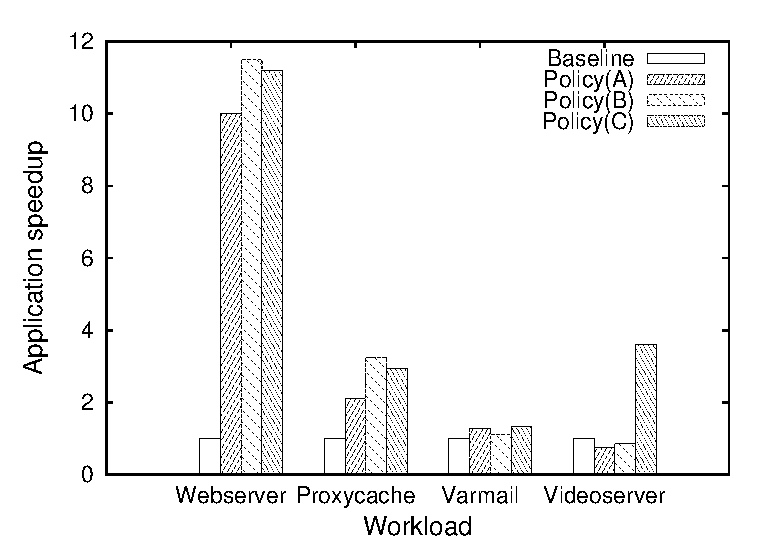
\includegraphics[width=0.55\textwidth]{speedup.eps}
 \caption{This is a bar graph showing the relative average speedup in the performance for multiple threads vs single thread , for different number of elements}
 \label{fig:speedup}
\end{figure}

\begin{figure}
\centering
\includegraphics[width=0.55\textwidth]{errorbar.eps}
 \caption{This is a bar graph showing the average speedup with error bars being the variances in the runtime for different number of elements , and for different number of threads}
 \label{fig:errorbar}
\end{figure}

\end{document}
